\chapter{Fermions, matrices de Dirac et mer de Dirac}

La mer de Dirac est notre destination, mais le chemin compte. Avant d’aborder l’énergie négative dans la théorie relativiste de l’électron, nous avons besoin de deux outils. Nous commencerons par l’algèbre des opérateurs qui distingue les fermions des bosons. Nous reverrons ensuite l’équation de Dirac à une dimension, où l’on peut observer chaque élargissement de la fonction d’onde sans la géométrie des trois dimensions spatiales. Une fois ces éléments en place, l’équation tridimensionnelle imposera sa propre structure matricielle, et la discussion initiale des états fermioniques occupés et inoccupés reviendra comme clé de compréhension des positrons.

Nous posons \(c=\hbar=1\). La lettre majuscule \(P\) désigne un opérateur impulsion, la lettre minuscule \(p\) une valeur propre de l’impulsion, et les symboles en gras leurs versions tridimensionnelles.

\section{L’échange devient une algèbre d’opérateurs}

Considérons deux particules identiques, l’une en \(x\), l’autre en \(y\). Les étiquettes \(x\) et \(y\) désignent des positions complètes ; ce ne sont pas deux coordonnées cartésiennes d’une seule particule. L’action de deux opérateurs de création sur le vide donne
\begin{equation}
\lvert x,y\rangle
=
\psi^\dagger(x)\psi^\dagger(y)\lvert0\rangle.
\label{eq:l10-two-particle-state}
\end{equation}

Pour des bosons, l’échange des deux places laisse l’état inchangé :
\begin{equation}
\lvert x,y\rangle=\lvert y,x\rangle.
\end{equation}
L’énoncé en termes d’opérateurs qui garantit cette symétrie est
\begin{equation}
\psi^\dagger(x)\psi^\dagger(y)
=
\psi^\dagger(y)\psi^\dagger(x).
\label{eq:l10-boson-exchange}
\end{equation}
Deux opérateurs de création bosoniques commutent ; on peut donc inverser leur ordre sans changer l’état qu’ils créent.

Pour des fermions, l’échange change le signe :
\begin{equation}
\lvert x,y\rangle=-\lvert y,x\rangle.
\label{eq:l10-fermion-state-exchange}
\end{equation}
Le signe global d’un vecteur d’état isolé n’est pas observable, mais les signes relatifs entre plusieurs possibilités le sont ; il faut donc conserver ce signe moins de manière cohérente. L’équation~\eqref{eq:l10-fermion-state-exchange} impose
\begin{equation}
\psi^\dagger(x)\psi^\dagger(y)
=
-\,\psi^\dagger(y)\psi^\dagger(x).
\label{eq:l10-fermion-operator-exchange}
\end{equation}

\begin{figure}[htbp]
\centering
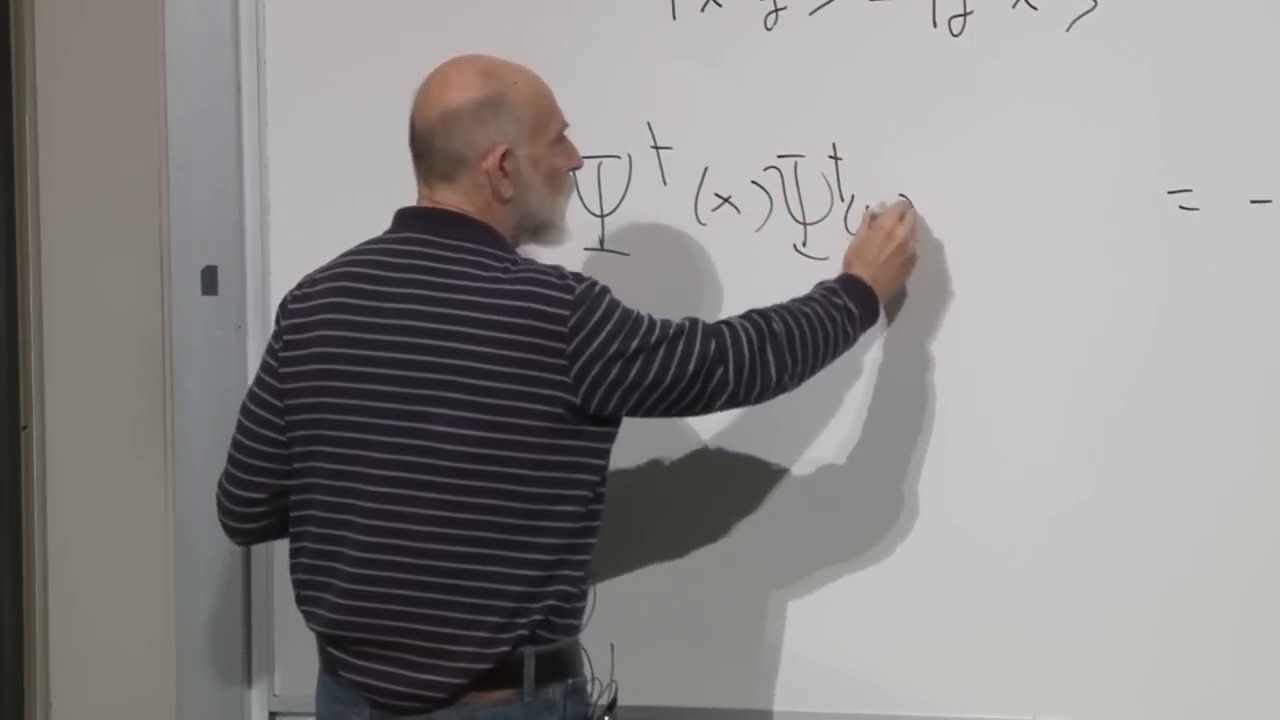
\includegraphics[width=0.94\linewidth]{lecture_10_figure_02.png}
\caption{La relation d’échange fermionique inscrite au tableau. L’inversion de l’ordre des opérateurs de création change le signe de l’état à deux particules.}
\lectureframe{00:05:50}
\end{figure}

Pour deux opérateurs quelconques \(A\) et \(B\), définissons l’anticommutateur par
\begin{equation}
\{A,B\}:=AB+BA.
\end{equation}
La règle d’échange s’écrit donc
\begin{equation}
\{\psi^\dagger(x),\psi^\dagger(y)\}=0.
\label{eq:l10-creation-anticommutator}
\end{equation}
L’algèbre correspondante des champs fermioniques remplace les commutateurs bosoniques par des anticommutateurs. Il faut distinguer les deux emplois du mot : les opérateurs de champ anticommutent en raison de la statistique de Fermi, tandis que les matrices anticommuteront plus tard afin d’annuler les termes croisés dans une relation de dispersion relativiste.

Posons maintenant \(y=x\) dans l’équation~\eqref{eq:l10-creation-anticommutator}. Les deux produits deviennent identiques :
\begin{align}
0
&=\{\psi^\dagger(x),\psi^\dagger(x)\}\\
&=2\,\psi^\dagger(x)\psi^\dagger(x).
\end{align}
Par conséquent,
\begin{equation}
\bigl(\psi^\dagger(x)\bigr)^2=0.
\label{eq:l10-exclusion}
\end{equation}
La tentative de créer deux fermions identiques dans le même état à une particule donne le vecteur nul. C’est le principe d’exclusion sous forme opératorielle.

\begin{figure}[htbp]
\centering
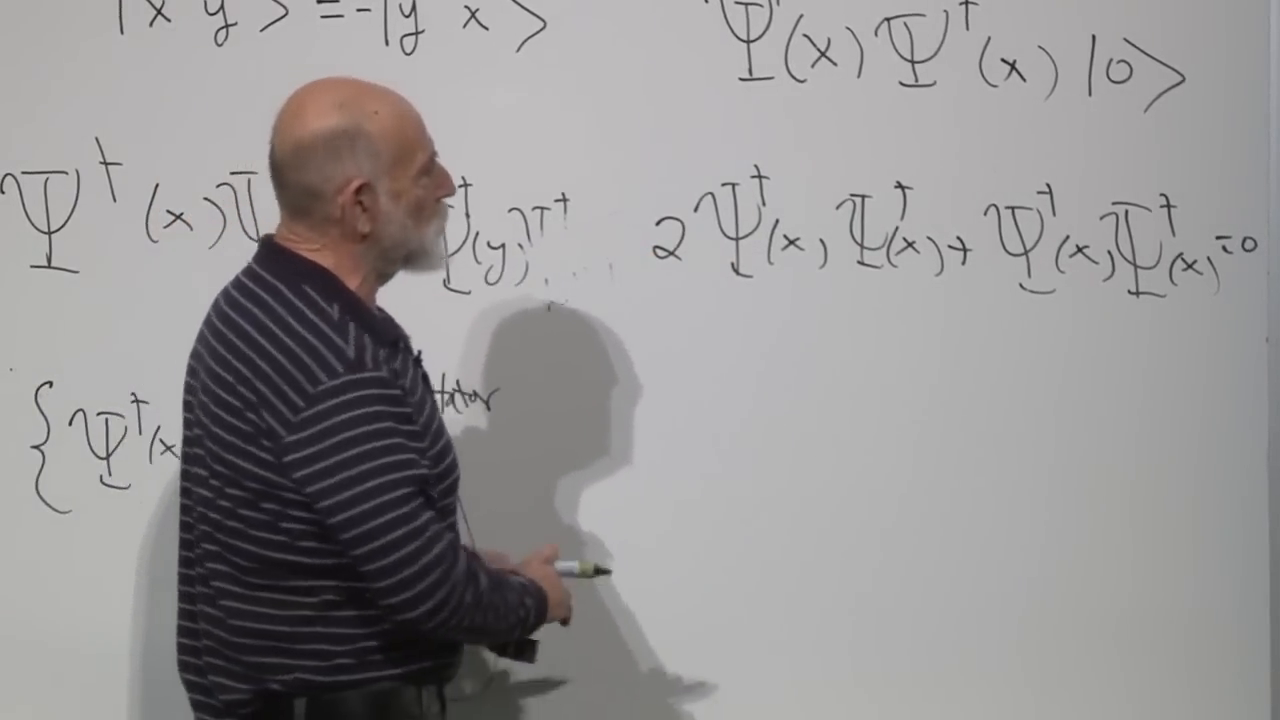
\includegraphics[width=0.94\linewidth]{lecture_10_figure_03.png}
\caption{Le cas particulier d’états identiques au tableau. Le produit répété d’opérateurs de création apparaît deux fois et doit donc s’annuler.}
\lectureframe{00:08:04}
\end{figure}

\begin{figure}[htbp]
\centering
\begin{adjustbox}{max width=\linewidth}
\begin{tikzpicture}[node distance=1.25cm,>=Latex]
\node[draw,rounded corners,align=center,inner sep=7pt] (a)
  {$\{\psi^\dagger(x),\psi^\dagger(x)\}=0$};
\node[draw,rounded corners,align=center,inner sep=7pt,right=of a] (b)
  {$2(\psi^\dagger(x))^2=0$};
\node[draw,rounded corners,align=center,inner sep=7pt,right=of b] (c)
  {$(\psi^\dagger(x))^2=0$};
\draw[->,thick] (a) -- (b);
\draw[->,thick] (b) -- (c);
\end{tikzpicture}
\end{adjustbox}
\caption{La démonstration de l’exclusion reconstituée sans les étapes intermédiaires partiellement effacées du tableau.}
\end{figure}

\section{Pourquoi l’occupation et l’absence d’occupation sont symétriques pour un fermion}

Il existe une autre différence entre les opérateurs bosoniques et fermioniques, plus subtile que l’exclusion et essentielle pour la suite. Pour un mode bosonique unique,
\begin{equation}
[a,a^\dagger]=1,
\qquad
n=0,1,2,\ldots.
\end{equation}
L’inversion de l’ordre de \(a\) et \(a^\dagger\) change le signe du commutateur. Même si l’on appelait simplement les opérateurs \(A\) et \(B\), l’algèbre nous indiquerait lequel augmente le nombre d’occupation et lequel le diminue.

L’échelle d’occupation bosonique a aussi une orientation. L’opérateur d’annihilation finit par atteindre \(\lvert0\rangle\) et donne zéro, tandis que l’opérateur de création peut continuer indéfiniment :
\begin{align}
a\lvert0\rangle&=0,\\
a^\dagger\lvert n\rangle&\propto\lvert n+1\rangle,
\qquad n=0,1,2,\ldots.
\end{align}
Retourner cette échelle ne reproduit pas le même spectre. Il y a un minimum, mais pas de maximum.

Pour un mode fermionique unique,
\begin{equation}
\{a,a^\dagger\}=1,
\qquad
a^2=(a^\dagger)^2=0,
\qquad
n=0,1.
\label{eq:l10-fermion-mode}
\end{equation}
L’opérateur de création fait passer de l’état inoccupé à l’état occupé, puis s’arrête :
\begin{equation}
a^\dagger\lvert0\rangle=\lvert1\rangle,
\qquad
a^\dagger\lvert1\rangle=0.
\end{equation}
L’opérateur d’annihilation effectue l’opération inverse :
\begin{equation}
a\lvert1\rangle=\lvert0\rangle,
\qquad
a\lvert0\rangle=0.
\end{equation}
Il n’y a que deux états ; le diagramme est donc symétrique si l’on échange l’état occupé et l’état inoccupé, ainsi que \(a\) et \(a^\dagger\). Les opérateurs gardent des significations physiques différentes, mais leur algèbre ne distingue plus l’un comme opérateur de création et l’autre comme opérateur d’annihilation. Cette symétrie formelle est à l’origine de la réinterprétation en termes de particule-trou.

\begin{classroomqa}
\lecturetimestamp{00:13:54}
\audiencequestion{Si \((a^\dagger)^2=0\), est-ce contradictoire, ou cela implique-t-il que \(a^\dagger=0\) ?}
\lecturerresponse{Ni l’un ni l’autre. Un opérateur non nul peut avoir un carré nul. Ici, \(a^\dagger\) fait passer \(\lvert0\rangle\) à \(\lvert1\rangle\), mais aucun état autorisé ne se trouve au-dessus de \(\lvert1\rangle\) ; une seconde application donne donc zéro. Le même raisonnement donne \(a^2=0\).}
\end{classroomqa}

Gardons cette symétrie entre état occupé et état inoccupé à l’esprit. Lorsqu’un électron d’énergie négative sera retiré, l’opérateur d’annihilation sera renommé opérateur de création de positron. Ce changement n’est pas une modification arbitraire de la notation : il repose précisément sur l’algèbre fermionique à deux états établie ici.

\section{La construction de Dirac à une dimension}

Revenons maintenant à une particule dans une seule dimension spatiale. L’équation d’onde relativiste du premier ordre la plus simple est
\begin{equation}
i\partial_t\psi=-\,i\partial_x\psi.
\label{eq:l10-right-mover}
\end{equation}
Avec \(P=-i\partial_x\), on obtient
\begin{equation}
H=P.
\end{equation}
Un état propre de l’impulsion vérifie \(E=p\), et sa vitesse de groupe est
\begin{equation}
v_g=\frac{dE}{dp}=1.
\end{equation}
Que l’impulsion, et donc l’énergie, soit positive ou négative, l’onde se propage toujours vers la droite sans se déformer. Le signe de \(p\) modifie la structure de phase, pas le sens de propagation.

Une particule massive doit pouvoir se déplacer dans les deux sens. Introduisons une seconde composante qui vérifie
\begin{equation}
H\psi_1=P\psi_1,
\qquad
H\psi_2=-P\psi_2.
\label{eq:l10-two-directions}
\end{equation}
La première composante se propage vers la droite ; la seconde, vers la gauche. Regroupons-les dans une colonne,
\begin{equation}
\Psi=
\begin{pmatrix}
\psi_1\\
\psi_2
\end{pmatrix},
\end{equation}
et définissons
\begin{equation}
\alpha=
\begin{pmatrix}
1&0\\
0&-1
\end{pmatrix}.
\end{equation}
Les deux équations deviennent
\begin{equation}
H\Psi=\alpha P\Psi.
\label{eq:l10-massless-one-d}
\end{equation}
Inclure les deux sens de propagation a pour contrepartie l’introduction d’un nouveau degré de liberté interne à deux valeurs.

Le seul sens de propagation ne produit pas la masse. Introduisons une seconde matrice,
\begin{equation}
\beta=
\begin{pmatrix}
0&1\\
1&0
\end{pmatrix},
\end{equation}
et essayons
\begin{equation}
H=\alpha P+\beta m.
\label{eq:l10-massive-one-d}
\end{equation}
Les matrices vérifient
\begin{equation}
\alpha^2=\beta^2=\mathbb{1},
\qquad
\{\alpha,\beta\}=0.
\label{eq:l10-one-d-algebra}
\end{equation}
En élevant le Hamiltonien au carré, on obtient
\begin{align}
H^2
&=(\alpha P+\beta m)^2\\
&=\alpha^2P^2+\beta^2m^2
  +(\alpha\beta+\beta\alpha)Pm\\
&=P^2+m^2.
\label{eq:l10-one-d-dispersion}
\end{align}
L’anticommutateur de l’équation~\eqref{eq:l10-one-d-algebra} élimine le terme indésirable, linéaire à la fois en \(P\) et en \(m\).

La matrice hors diagonale \(\beta\) couple les deux composantes associées aux sens de propagation. On peut se représenter le terme de masse comme un mélange continu des amplitudes se propageant vers la droite et vers la gauche. Il ne faut pas prendre cette image au pied de la lettre, comme si la particule rebondissait le long d’une trajectoire microscopique ; elle permet toutefois de comprendre pourquoi un paquet d’ondes massif peut avoir une vitesse moyenne inférieure à celle de la lumière et posséder un référentiel de repos, contrairement à une composante chirale sans masse isolée.

\begin{classroomqa}
\lecturetimestamp{00:23:37}
\audiencequestion{L’introduction de deux composantes associées aux sens de propagation a-t-elle une interprétation physique plus profonde ?}
\lecturerresponse{Oui, mais elle apparaît plus clairement en trois dimensions. À ce stade, il s’agit simplement des deux composantes nécessaires pour décrire les sens de propagation opposés et permettre un couplage de masse hors diagonale. Leur interprétation ultérieure sera la chiralité.}
\end{classroomqa}

\section{Les trois dimensions imposent les matrices de Pauli}

En trois dimensions spatiales, l’impulsion est un vecteur. Un Hamiltonien linéaire en l’impulsion et scalaire sous les rotations suggère donc un autre vecteur, dont les composantes sont cette fois des matrices :
\begin{equation}
H=\boldsymbol{\alpha}\cdot\mathbf P
=\alpha_xP_x+\alpha_yP_y+\alpha_zP_z.
\label{eq:l10-three-d-ansatz}
\end{equation}

\begin{figure}[htbp]
\centering
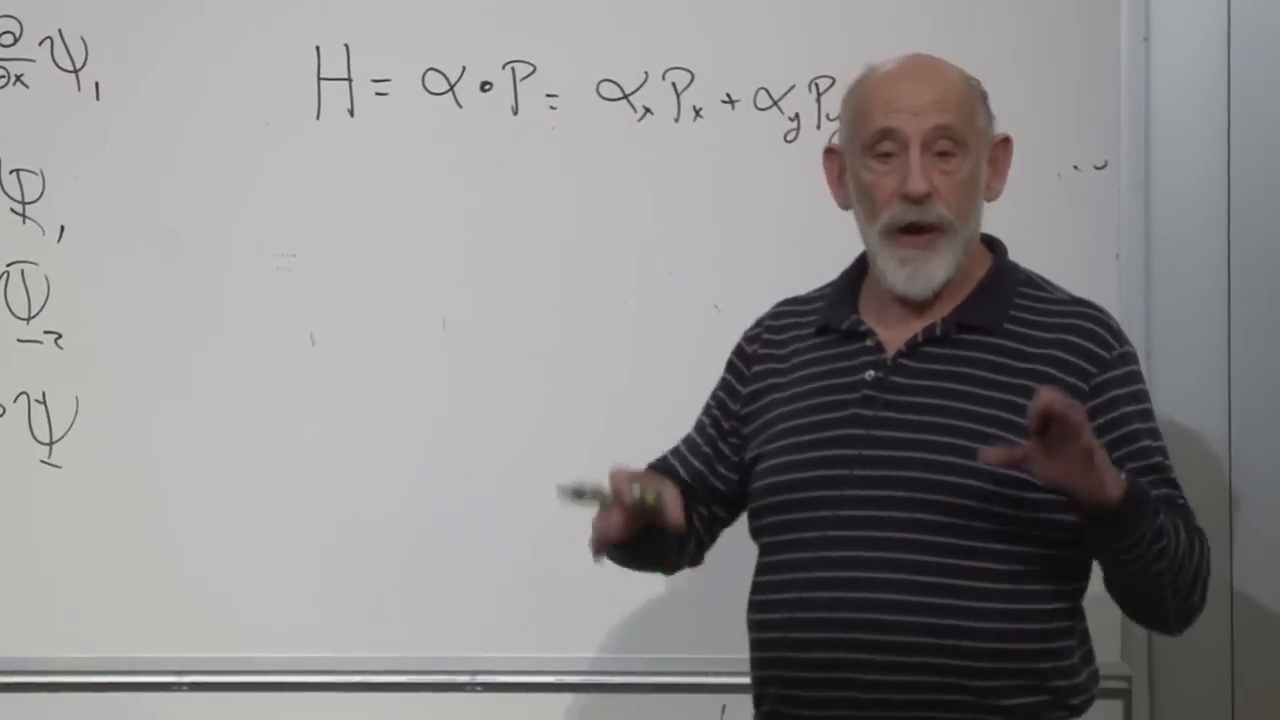
\includegraphics[width=0.94\linewidth]{lecture_10_figure_04.png}
\caption{L’ansatz sans masse tridimensionnel \(H=\boldsymbol{\alpha}\cdot\mathbf P\), au moment où une matrice devient un vecteur de trois matrices.}
\lectureframe{00:26:00}
\end{figure}

Repartons du cas sans masse. Nous imposons
\begin{equation}
H^2=\mathbf P^2=P_x^2+P_y^2+P_z^2.
\end{equation}
En développant le carré de l’équation~\eqref{eq:l10-three-d-ansatz},
\begin{align}
H^2
&=\alpha_x^2P_x^2+\alpha_y^2P_y^2\\
&\quad+\alpha_z^2P_z^2\\
&\quad+\{\alpha_x,\alpha_y\}P_xP_y\\
&\quad+\{\alpha_x,\alpha_z\}P_xP_z\\
&\quad+\{\alpha_y,\alpha_z\}P_yP_z.
\end{align}
Les termes diagonaux sont corrects si
\begin{equation}
\alpha_x^2=\alpha_y^2=\alpha_z^2=\mathbb{1},
\end{equation}
et tous les termes croisés s’annulent si
\begin{equation}
\{\alpha_i,\alpha_j\}=0,
\qquad i\ne j.
\label{eq:l10-alpha-anticommutation}
\end{equation}

Trois matrices \(2\times2\) bien connues satisfont précisément ces conditions :
\begin{equation}
\sigma_x=
\begin{pmatrix}
0&1\\
1&0
\end{pmatrix},
\quad
\sigma_y=
\begin{pmatrix}
0&-i\\
i&0
\end{pmatrix},
\quad
\sigma_z=
\begin{pmatrix}
1&0\\
0&-1
\end{pmatrix}.
\label{eq:l10-pauli-matrices}
\end{equation}
Une solution est donc
\begin{equation}
\alpha_i=\sigma_i,
\qquad
H=\boldsymbol{\sigma}\cdot\mathbf P.
\label{eq:l10-weyl-hamiltonian}
\end{equation}

\begin{figure}[htbp]
\centering
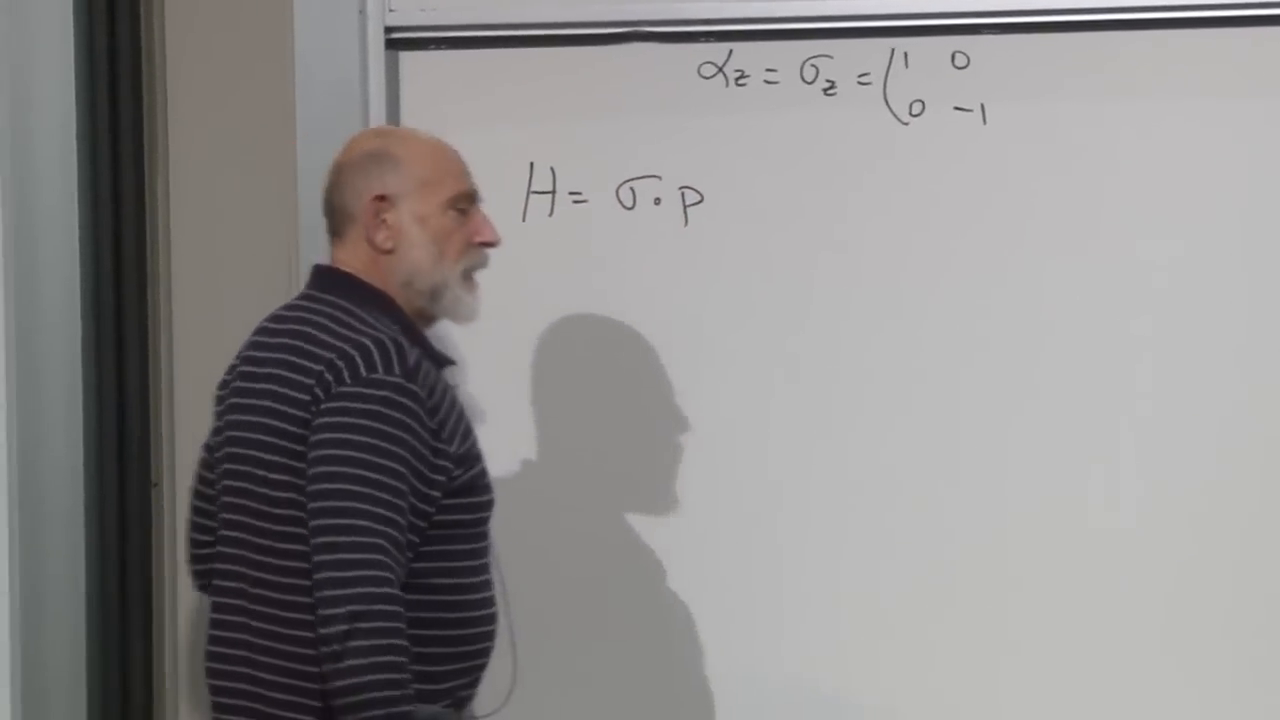
\includegraphics[width=0.94\linewidth]{lecture_10_figure_05.png}
\caption{Le Hamiltonien sans masse sous forme compacte \(H=\boldsymbol{\sigma}\cdot\mathbf P\), avec \(\alpha_z=\sigma_z\) encore visible au-dessus.}
\lectureframe{00:28:16}
\end{figure}

Pour un état propre de l’impulsion,
\begin{equation}
\boldsymbol{\sigma}\cdot\mathbf p
=
|\mathbf p|\,\boldsymbol{\sigma}\cdot\widehat{\mathbf p}.
\end{equation}
L’opérateur \(\boldsymbol{\sigma}\cdot\widehat{\mathbf p}\) a pour valeurs propres \(+1\) et \(-1\), donc
\begin{equation}
E=\pm|\mathbf p|.
\end{equation}
Dans cette théorie à deux composantes, pour une énergie positive, le degré de liberté de Pauli est aligné sur l’impulsion ; pour une énergie négative, il lui est anti-aligné. Cet alignement est fixé : pour un signe d’énergie donné, la direction du spin ne peut pas être réglée indépendamment.

\begin{classroomqa}
\lecturetimestamp{00:30:10}
\audiencequestion{Le spin découle-t-il de l’équation de Dirac, ou a-t-il été introduit parce que l’on sait déjà que l’électron possède un moment magnétique ?}
\lecturerresponse{Ici, « découler » signifie « apparaître comme conséquence », et non « disparaître ». Le point de départ était l’exigence d’un Hamiltonien linéaire en l’impulsion dont le carré soit \(\mathbf P^2\). Des nombres ordinaires ne peuvent satisfaire l’algèbre requise, contrairement aux matrices de Pauli. Leur structure à deux composantes apparaît donc dès la linéarisation. Cela ne prouve pas que toute particule doit avoir un spin ; cela signifie que les particules décrites par cette équation de type Dirac portent le degré de liberté spinoriel correspondant.}
\end{classroomqa}

C’est l’une des leçons centrales de cette construction. Les matrices ne sont pas des étiquettes décoratives ajoutées après avoir trouvé l’équation relativiste. C’est la tentative de prendre une racine carrée locale de la relation de dispersion relativiste qui les fait apparaître.

\section{Pourquoi la masse exige quatre composantes}

Essayons de reprendre la construction de la masse à une dimension sans élargir la théorie \(2\times2\) :
\begin{equation}
H=\boldsymbol{\sigma}\cdot\mathbf P+\beta m.
\label{eq:l10-failed-mass}
\end{equation}
Supposons \(\beta^2=\mathbb{1}\). Le carré contient les termes voulus \(\mathbf P^2+m^2\), mais aussi
\begin{equation}
m\sum_i\{\sigma_i,\beta\}P_i.
\end{equation}
Pour éliminer ce terme, une matrice \(\beta\) devrait vérifier
\begin{equation}
\{\sigma_x,\beta\}
=
\{\sigma_y,\beta\}
=
\{\sigma_z,\beta\}
=0.
\label{eq:l10-impossible-beta}
\end{equation}
Aucune matrice \(2\times2\) ne le peut. L’identité commute avec les trois matrices de Pauli, et toute matrice \(2\times2\) sans trace est une combinaison linéaire de matrices de Pauli. Aucune combinaison de ce type n’anticommute avec la composante qui lui est parallèle. L’algèbre \(2\times2\) ne contient pas de quatrième matrice indépendante répondant à la condition requise.

La solution consiste à élargir le spineur. Quatre matrices qui anticommuttent deux à deux et dont les carrés sont l’identité apparaissent pour la première fois dans une représentation complexe \(4\times4\). Cette taille de matrice n’est pas choisie parce que l’espace-temps a quatre dimensions ; c’est le plus petit espace matriciel capable de réaliser l’algèbre requise.

Il existe de nombreuses représentations équivalentes. Un changement unitaire de base du spineur modifie les éléments de toutes les matrices sans changer aucune prédiction physique. Ce qui importe, c’est l’ensemble abstrait des relations
\begin{equation}
\{\alpha_i,\alpha_j\}=2\delta_{ij}\mathbb{1},
\qquad
\{\alpha_i,\beta\}=0,
\qquad
\beta^2=\mathbb{1}.
\label{eq:l10-dirac-algebra}
\end{equation}

\begin{classroomqa}
\lecturetimestamp{00:37:38}
\audiencequestion{Peut-on considérer \(\beta\) comme une composante temporelle \(\alpha_t\) ?}
\lecturerresponse{Pas directement. Les trois \(\alpha_i\) ne se combinent pas avec \(\beta\) pour former les quatre composantes d’un même vecteur de Lorentz. En notation covariante, on définit plutôt \(\beta=\gamma^0\) et \(\alpha_i=\gamma^0\gamma^i\) ; les quatre matrices \(\gamma^\mu\) satisfont l’algèbre de Clifford de l’espace-temps.}
\end{classroomqa}

Une représentation par blocs commode est
\begin{equation}
\alpha_i=
\begin{pmatrix}
\sigma_i&0\\
0&-\sigma_i
\end{pmatrix},
\qquad
\beta=
\begin{pmatrix}
0&I_2\\
I_2&0
\end{pmatrix}.
\label{eq:l10-block-representation}
\end{equation}
Les matrices de Pauli dans les blocs diagonaux garantissent que les différentes matrices \(\alpha_i\) anticommuttent. Les blocs d’identité hors diagonale de \(\beta\) garantissent que \(\beta\) anticommute avec chacune des matrices \(\alpha_i\).

\begin{figure}[htbp]
\centering
\includegraphics[width=0.94\linewidth]{lecture_10_figure_06.png}
\caption{La représentation par blocs \(4\times4\) inscrite au tableau. Les équations du haut indiquent les anticommutateurs requis ; les matrices complètes sont composées dans l’équation~\eqref{eq:l10-block-representation}.}
\lectureframe{00:41:10}
\end{figure}

Le Hamiltonien massif s’écrit maintenant
\begin{equation}
H=\boldsymbol{\alpha}\cdot\mathbf P+\beta m
=
\begin{pmatrix}
\boldsymbol{\sigma}\cdot\mathbf P&mI_2\\
mI_2&-\boldsymbol{\sigma}\cdot\mathbf P
\end{pmatrix}.
\label{eq:l10-massive-dirac}
\end{equation}
En utilisant l’équation~\eqref{eq:l10-dirac-algebra},
\begin{equation}
H^2=\mathbf P^2+m^2.
\end{equation}
La structure à quatre composantes n’est donc pas un ajout facultatif. C’est la structure minimale permettant d’inclure à la fois l’impulsion tridimensionnelle et un terme de masse tout en conservant une équation du premier ordre.

\section{La chiralité et le sens des composantes supplémentaires}

Quelle distinction physique l’élargissement a-t-il introduite ? Partons du bloc supérieur sans masse,
\begin{equation}
H_R=\boldsymbol{\sigma}\cdot\mathbf P,
\end{equation}
et du bloc inférieur sans masse,
\begin{equation}
H_L=-\boldsymbol{\sigma}\cdot\mathbf P.
\end{equation}
Pour les états d’énergie positive, le spin du premier est aligné sur l’impulsion, tandis que celui du second lui est anti-aligné. Ce sont des hélicités opposées. Dans une théorie sans masse, l’hélicité est invariante sous les transformations de Lorentz propres, car aucun observateur ne peut dépasser une particule de genre lumière et inverser son impulsion tout en laissant son spin inchangé. Les deux blocs décrivent donc des secteurs de chiralité opposée.

\begin{classroomqa}
\lecturetimestamp{00:41:28}
\audiencequestion{À une dimension, un degré de liberté binaire supplémentaire était nécessaire pour introduire la masse. Quelle distinction physique lui correspond en trois dimensions ?}
\lecturerresponse{Il s’agit de la chiralité du spineur. Les deux blocs \(2\times2\) portent des relations opposées entre le spin et l’impulsion. L’un est droitier, l’autre gaucher. La théorie \(4\times4\) contient les deux.}
\end{classroomqa}

Le terme de masse de l’équation~\eqref{eq:l10-massive-dirac} est hors diagonale. Il transforme une amplitude du bloc supérieur en une amplitude du bloc inférieur, et inversement :
\begin{equation}
\beta m
\begin{pmatrix}
\Psi_R\\
\Psi_L
\end{pmatrix}
=
m
\begin{pmatrix}
\Psi_L\\
\Psi_R
\end{pmatrix}.
\end{equation}
La masse couple donc les chiralités opposées.

\begin{classroomqa}
\lecturetimestamp{00:43:58}
\audiencequestion{Une particule sans masse peut-elle changer de chiralité ?}
\lecturerresponse{Pas avec le Hamiltonien libre sans masse présenté ici. Les deux blocs sont découplés ; un état initialement droitier ou gaucher le reste. Le terme de masse hors diagonale est précisément ce qui les mélange lorsque \(m\ne0\).}
\end{classroomqa}

Cette terminologie est exacte pour la représentation par blocs, mais il ne faut pas pousser trop loin l’image d’une particule qui basculerait mécaniquement entre deux flèches. L’énoncé physique est le couplage matriciel dans l’équation d’onde.

\begin{classroomqa}
\lecturetimestamp{00:44:50}
\audiencequestion{Ces matrices sont-elles intégrées aux quaternions ?}
\lecturerresponse{Les matrices de Pauli sont étroitement liées aux unités quaternioniques : les matrices \(-i\sigma_i\) ont pour carré \(-\mathbb{1}\) et se multiplient selon la structure quaternionique, à des conventions d’orientation près. Les matrices de Dirac complètes nécessitent l’algèbre de Clifford de dimension supérieure, et le lien avec les quaternions n’est pas nécessaire pour la suite du raisonnement.}
\end{classroomqa}

\begin{classroomqa}
\lecturetimestamp{00:46:34}
\audiencequestion{Si le spin est un moment cinétique, y a-t-il ici un terme d’énergie qui lui est associé ?}
\lecturerresponse{Aucun terme indépendant pour une particule libre n’est ajouté. La structure spinorielle intervient déjà dans le Hamiltonien cinétique par l’intermédiaire des matrices. Le couplage du spin à un champ magnétique extérieur introduirait des termes d’interaction supplémentaires, mais c’est un autre problème.}
\end{classroomqa}

\section{Les matrices alpha représentent la vitesse, pas le spin}

Chaque matrice \(\alpha_i\) a deux valeurs propres \(+1\) et deux valeurs propres \(-1\). Les différentes composantes ne commutent pas ; elles ne peuvent donc pas toutes être mesurées simultanément avec précision. Pour déterminer ce que représente une composante, utilisons l’équation de Heisenberg. Pour un opérateur \(L\) sans dépendance temporelle explicite,
\begin{equation}
\dot L=i[H,L].
\label{eq:l10-heisenberg}
\end{equation}
La convention de signe est fixée ici par l’évolution Schr\"odinger \(e^{-iHt}\).

Appliquons l’équation~\eqref{eq:l10-heisenberg} à l’opérateur position \(x\). Les matrices agissent sur les indices du spineur et commutent avec la position ; seul \(P_x\) ne commute pas avec \(x\) :
\begin{align}
\dot x
&=i[\boldsymbol{\alpha}\cdot\mathbf P+\beta m,x]\\
&=i\alpha_x[P_x,x]\\
&=\alpha_x,
\label{eq:l10-velocity}
\end{align}
car \([P_x,x]=-i\). Ainsi, \(\alpha_x\) est la composante \(x\) de l’opérateur vitesse ; de même,
\begin{equation}
\dot{\mathbf x}=\boldsymbol{\alpha}.
\end{equation}

\begin{classroomqa}
\lecturetimestamp{00:51:50}
\audiencequestion{Une mesure d’une composante de la vitesse ne donne-t-elle vraiment que \(+1\) ou \(-1\) ?}
\lecturerresponse{Oui, pour l’opérateur instantané \(\alpha_i\) dans les unités \(c=1\). Un état général n’est pas nécessairement un état propre ; sa valeur moyenne peut donc se situer n’importe où entre ces valeurs. Le paquet d’ondes qui se propage de façon régulière a une vitesse moyenne inférieure à celle de la lumière lorsque la particule est massive.}
\end{classroomqa}

La vitesse n’est pas conservée :
\begin{equation}
\dot\alpha_x=i[H,\alpha_x]\ne0.
\end{equation}
Les termes contenant \(\alpha_y\), \(\alpha_z\) et \(\beta\) ne commutent pas avec \(\alpha_x\). Un état comportant des composantes d’énergie positive et négative présente donc une contribution rapidement oscillante à sa position. C’est le \emph{tremblement de Zitterbewegung}, littéralement un mouvement de tremblement.

Après moyenne sur des durées longues devant la période de l’oscillation rapide, la vitesse relativiste moyenne attendue est
\begin{equation}
\overline{\mathbf v}=\frac{\mathbf p}{E},
\end{equation}
ce qui se réduit à \(\mathbf p/m\) pour un électron lent.

\begin{classroomqa}
\lecturetimestamp{00:54:40}
\audiencequestion{Un électron libre qui tremble sans force extérieure viole-t-il la loi de Newton ?}
\lecturerresponse{Non. L’invariance par translation conserve l’impulsion, donc \(\dot{\mathbf P}=0\). L’opérateur vitesse de Dirac n’est pas simplement \(\mathbf P/m\), et sa partie rapidement oscillante peut varier alors que l’impulsion reste constante. Le mouvement moyenné dans le temps obéit à la relation attendue pour une particule libre.}
\end{classroomqa}

\begin{classroomqa}
\lecturetimestamp{00:55:22}
\audiencequestion{La vitesse vaut-elle toujours \(c\) ?}
\lecturerresponse{Une mesure instantanée d’une composante \(\alpha_i\) a pour valeurs propres \(\pm c\), mais un paquet d’ondes massif est généralement une superposition et sa valeur moyenne est subluminale. Sa vitesse de groupe moyenne est \(\mathbf p/E\).}
\end{classroomqa}

\begin{classroomqa}
\lecturetimestamp{00:55:30}
\audiencequestion{Peut-on se représenter l’oscillation comme une variation de la vitesse due à la masse ?}
\lecturerresponse{Non. La masse est un paramètre fixe. L’oscillation provient de la non-commutation des opérateurs vitesse et Hamiltonien, ou, de façon équivalente, de l’interférence entre les secteurs d’énergie ; elle ne résulte pas d’une masse fluctuante.}
\end{classroomqa}

\begin{classroomqa}
\lecturetimestamp{00:56:22}
\audiencequestion{Une mesure instantanée peut-elle trouver une vitesse orientée dans un sens alors que le mouvement moyen s’oriente dans un autre ?}
\lecturerresponse{Oui. L’opérateur de composante possède les deux valeurs propres nettes, tandis que des mesures répétées ou moyennées dans le temps retrouvent la dérive plus régulière.}
\end{classroomqa}

Il faut aussi employer le mot spin avec précision. Les matrices \(\alpha_i\) se transforment comme les composantes de la vitesse, un vecteur ordinaire. Le véritable opérateur de spin dans cette représentation est
\begin{equation}
\mathbf S=\frac12\boldsymbol{\Sigma},
\qquad
\Sigma_i=
\begin{pmatrix}
\sigma_i&0\\
0&\sigma_i
\end{pmatrix}.
\label{eq:l10-spin-operator}
\end{equation}
Il diffère de \(\alpha_i\) par le signe du bloc inférieur. Ces matrices sont étroitement liées, mais la vitesse et le spin ne sont pas la même observable.

\section{Énergie négative et vide d’énergie minimale}

Le problème de l’énergie négative se pose déjà avant toute cette machinerie matricielle. Revenons au mode se propageant vers la droite à une dimension,
\begin{equation}
H=P.
\end{equation}
Puisque \(p\) parcourt toute la droite réelle, \(E=p\) n’est pas minorée.

Le vide ne peut pas simplement désigner un état sans particules. Il doit être l’état à partir duquel on ne peut plus retirer d’énergie. Si un état vide nous permet d’ajouter une particule d’énergie négative, d’abaisser l’énergie, d’en ajouter une autre et de continuer indéfiniment, alors cet état vide n’est pas un vide stable.

La statistique de Fermi offre une solution historique. Plaçons un électron dans chaque état d’énergie négative. Chaque électron ajouté abaisse l’énergie totale, mais le principe d’exclusion n’autorise qu’un électron par état à une particule. Une fois tous les états d’énergie négative occupés, aucun électron supplémentaire ne peut tomber dans ce secteur. Dirac a identifié cette configuration remplie au vide.

La même construction échouerait pour des bosons. Un nombre arbitrairement grand de bosons peut occuper un seul état ; un mode bosonique d’énergie négative pourrait donc absorber des particules sans limite. La borne fermionique \(n=0,1\), introduite au début du cours, est précisément ce qui arrête la chute.

\begin{figure}[htbp]
\centering
\includegraphics[width=0.94\linewidth]{lecture_10_figure_07.png}
\caption{La représentation historique de la mer de Dirac au tableau : une échelle de niveaux d’énergie négative remplis jusqu’à la ligne de séparation, avec les états d’énergie positive au-dessus.}
\lectureframe{01:02:45}
\end{figure}

\begin{figure}[htbp]
\centering
\begin{adjustbox}{max width=\linewidth}
\begin{tikzpicture}[x=1.05cm,y=0.72cm,>=Latex]
\draw[->] (0,-4.8) -- (0,4.8) node[above] {$E$};
\draw[thick] (-2.9,0) -- (3.2,0) node[right] {$E=0$};
\foreach \y in {-4,-3.3,...,-0.5} {
  \draw (-2.3,\y) -- (2.3,\y);
  \foreach \x in {-1.8,-1.2,...,1.8} {
    \fill[blue!65!black] (\x,\y) circle (1.6pt);
  }
}
\foreach \y in {0.8,1.6,...,4.0} {
  \draw (-2.3,\y) -- (2.3,\y);
}
\draw[red,very thick] (0.6,-2.6) circle (5pt);
\draw[red,->,very thick] (0.6,-2.35) .. controls (1.4,-0.4) and (1.2,1.6) .. (1.5,2.4);
\fill[red] (1.5,2.4) circle (2.5pt);
\node[right,red] at (0.85,-2.6) {hole};
\node[right,red] at (1.7,2.4) {$e^-$};
\node[left] at (-2.5,-2.2) {filled negative-energy states};
\end{tikzpicture}
\end{adjustbox}
\caption{Reconstitution claire d’une excitation au-dessus d’une mer remplie : la promotion d’un électron d’énergie négative laisse un trou d’énergie positive.}
\end{figure}

La mer est une image historique d’une réorganisation correcte des opérateurs. Il ne faut pas prendre sa charge et son énergie littéralement infinies pour des quantités directement observables ; la reformulation moderne évitera d’avoir à imaginer des électrons matériels remplissant l’espace.

\section{Un trou est un positron}

Lorsque tous les états d’énergie négative sont occupés, deux types d’excitation sont possibles. On peut ajouter un électron d’énergie positive au-dessus de la mer, ou retirer un électron d’énergie négative et laisser un trou.

Un trou porte la charge opposée à celle de l’électron manquant. Le retrait d’une charge \(-e\) modifie la charge de \(+e\). Il possède aussi une énergie d’excitation positive. Si l’électron retiré avait \(E_-<0\), l’énergie mesurée par rapport au vide rempli varie de
\begin{equation}
E_{\mathrm{hole}}=-E_->0.
\end{equation}
Le trou est une excitation d’énergie positive et de charge positive : le positron.

Un photon peut promouvoir un électron de la mer vers un état d’énergie positive. Par rapport au vide, l’état final contient un électron et un positron. Dans un diagramme ordonné dans le temps, on représente conventionnellement le flux du nombre d’électrons vers le haut pour l’électron, et la ligne du positron par une flèche de sens opposé. Les flèches indiquent le flux du nombre fermionique ou de la charge ; ce ne sont pas de petits vecteurs classiques de vitesse.

\begin{classroomqa}
\lecturetimestamp{01:05:14}
\audiencequestion{Cette image impose-t-elle un nombre égal d’électrons et de positrons ?}
\lecturerresponse{Pas pour un état quelconque. Si l’on part du vide et que l’on crée une paire neutre, on obtient une particule de chaque sorte, mais un état peut déjà contenir un excès d’électrons ou de positrons. La conservation de la charge contraint les réactions ; elle n’impose pas à chaque état autorisé des populations égales.}
\end{classroomqa}

Dirac ne savait pas, au départ, que le trou serait une particule de même masse que l’électron, ne différant de lui que par sa charge et d’autres nombres quantiques additifs. L’équation et la construction par les trous ont conduit à cette prédiction avant que le positron ne soit intégré au catalogue familier des particules.

\section{Un seul champ fermionique contient des électrons et des positrons}

L’opérateur de champ fait passer l’image historique dans le langage de l’algèbre moderne. Pour l’instant, omettons les indices spinoriels, les facteurs de normalisation et la dépendance temporelle. Un champ à une dimension peut être développé schématiquement sous la forme
\begin{equation}
\psi(x)
\sim
\int_{-\infty}^{\infty}dp\,a(p)e^{ipx}.
\label{eq:l10-full-field-integral}
\end{equation}
Pour la dispersion d’un mode se propageant vers la droite \(E=p\), les valeurs positives de \(p\) désignent une énergie positive et les valeurs négatives de \(p\) une énergie négative. Scindons l’intégrale :
\begin{equation}
\psi(x)
\sim
\int_0^\infty dp\,a(p)e^{ipx}
+
\int_{-\infty}^0 dp\,a(p)e^{ipx}.
\end{equation}
Dans le second terme, posons \(p=-q\), avec \(q>0\), puis réinterprétons l’annihilation d’un électron d’énergie négative de la mer remplie comme la création d’un positron :
\begin{equation}
b^\dagger(q):=a(-q).
\end{equation}
On obtient alors
\begin{equation}
\psi(x)
\sim
\int_0^\infty dp\,
\left[
a(p)e^{ipx}
+
b^\dagger(p)e^{-ipx}
\right].
\label{eq:l10-electron-positron-split}
\end{equation}
Les signes exacts des phases des ondes planes dépendent de la convention d’espace-temps ; le contenu invariant est que \(\psi\) contient un opérateur d’annihilation d’électron et un opérateur de création de positron.

\begin{figure}[htbp]
\centering
\includegraphics[width=0.94\linewidth]{lecture_10_figure_08.png}
\caption{L’intégrale du champ scindée en secteurs d’énergie positive et négative. La ligne du bas renomme l’opérateur d’électron d’énergie négative en opérateur de création de positron.}
\lectureframe{01:11:35}
\end{figure}

C’est ici que la symétrie entre état occupé et état inoccupé de l’équation~\eqref{eq:l10-fermion-mode} porte ses fruits. Pour les fermions, l’algèbre des opérateurs permet ce renommage sans modifier la structure des anticommutateurs.

Une interaction électromagnétique schématique prend la forme
\begin{equation}
H_{\mathrm{int}}
\sim
\int dx\,\psi^\dagger(x)\psi(x)A(x),
\label{eq:l10-qed-schematic}
\end{equation}
où \(A\) désigne le champ photonique. Comme chaque champ fermionique comporte des contributions d’électron et de positron, un seul opérateur local inclut plusieurs processus :
\begin{align}
e^-&\longrightarrow e^-+\gamma,\\
e^-+e^+&\longrightarrow\gamma,\\
\gamma&\longrightarrow e^-+e^+,
\end{align}
ainsi que leurs processus inverses et croisés. La conservation de l’énergie-impulsion détermine quel processus est cinématiquement possible dans un environnement donné. Par exemple, un photon réel isolé dans le vide ne peut pas créer une paire sans un autre participant qui absorbe le recul, même si le sommet local est présent dans l’interaction.

\begin{figure}[htbp]
\centering
\includegraphics[width=0.94\linewidth]{lecture_10_figure_09.png}
\caption{Le tableau juxtapose l’émission d’un électron, l’annihilation d’une paire et l’interaction schématique \(\psi^\dagger\psi A\). Différents choix parmi les mêmes opérateurs de champ engendrent les différents processus.}
\lectureframe{01:13:30}
\end{figure}

Un produit compact de champs organise donc de nombreuses réactions qui semblent différentes. Feynman a ensuite fourni les règles systématiques des diagrammes pour calculer les amplitudes, mais une grande partie de la structure opératorielle est déjà visible ici.

\section{Le langage moderne du vide et l’analogie avec la mer de Fermi}

\begin{classroomqa}
\lecturetimestamp{01:14:20}
\audiencequestion{Comment les physiciens modernes décrivent-ils cela sans traiter le vide comme une véritable mer de Dirac ?}
\lecturerresponse{Ils effectuent directement la réinterprétation des opérateurs. L’annihilation d’un électron d’énergie négative est renommée création d’un positron d’énergie positive, et le vide est défini comme l’état annihilé par tous les opérateurs d’annihilation d’électrons et de positrons. La formulation qui en résulte est symétrique entre particules et antiparticules et ne requiert aucune mer matérielle.}
\end{classroomqa}

La mer historique reste utile, car sa logique a un analogue étroit en matière condensée. Dans un cristal, un nombre fixe d’électrons occupent les états à une particule de plus basse énergie disponibles, jusqu’au niveau de Fermi. L’état fondamental rempli n’est pas vide. Promouvoir un électron au-dessus de ce niveau laisse un état inoccupé en dessous. Par rapport au fond rempli, le trou porte une énergie d’excitation positive et peut se comporter comme un porteur de charge positive.

Il existe des différences importantes. Un trou dans un solide vit dans un milieu, et sa masse effective ainsi que sa réponse à la charge dépendent de la structure de bandes. Un positron est une antiparticule élémentaire du champ quantique relativiste. Malgré cela, l’algèbre commune des particules et des trous rend l’analogie puissante.

\begin{classroomqa}
\lecturetimestamp{01:17:14}
\audiencequestion{La théorie de Klein--Gordon pour les bosons souffre-t-elle de la même cascade vers les états d’énergie négative ?}
\lecturerresponse{Non. Un champ complexe de Klein--Gordon quantifié correctement s’organise en particules et antiparticules d’énergie positive, sans qu’il soit nécessaire de remplir une mer bosonique. Son équation du second ordre et sa structure canonique diffèrent de la construction hamiltonienne de Dirac ; l’argument historique de la mer fermionique ne s’y transpose donc pas tel quel.}
\end{classroomqa}

\begin{classroomqa}
\lecturetimestamp{01:17:30}
\audiencequestion{D’où vient le spin 1 des bosons ?}
\lecturerresponse{Il ne vient pas de la linéarisation à l’aide des matrices de Pauli utilisée ici. Les champs de spin 1 ont leur propre loi de transformation de Lorentz et leurs propres équations de champ. La dérivation présentée ici explique la structure spinorielle des fermions de Dirac, et non tous les spins possibles des particules.}
\end{classroomqa}

\begin{classroomqa}
\lecturetimestamp{01:17:46}
\audiencequestion{Pourquoi la statistique de Fermi était-elle essentielle à la solution d’énergie négative ?}
\lecturerresponse{Parce que le principe d’exclusion limite l’occupation de chaque état à un électron. Une fois tous les états d’énergie négative occupés, aucun électron supplémentaire ne peut y tomber. L’occupation bosonique n’est soumise à aucune limite de ce type ; une mer littérale de bosons d’énergie négative n’aurait donc toujours pas de fond.}
\end{classroomqa}

\begin{classroomqa}
\lecturetimestamp{01:20:02}
\audiencequestion{La distinction entre électron et positron est-elle simplement un autre degré de liberté binaire, comme la charge ?}
\lecturerresponse{Pour compter les états, un champ de Dirac massif possède deux états de spin pour l’électron et deux pour le positron ; deux étiquettes binaires constituent donc un moyen mnémotechnique utile. Mais la distinction entre particule et antiparticule n’est pas un qubit interne que l’on pourrait faire tourner indépendamment pour un même électron : tous les électrons ont la charge \(-e\), tous les positrons la charge \(+e\), et cette distinction émerge des secteurs de fréquence positive et négative après quantification.}
\end{classroomqa}

La mer infinie soulève une dernière question.

\begin{classroomqa}
\lecturetimestamp{01:20:54}
\audiencequestion{La mer de Dirac infinie produirait-elle une constante cosmologique infinie ?}
\lecturerresponse{Elle met en évidence le problème de l’énergie du vide. Les modes bosoniques d’énergie du point zéro contribuent \(+\tfrac12\hbar\omega\), tandis que les modes fermioniques contribuent avec le signe opposé. Des compensations formelles sont possibles lorsque les spectres coïncident, mais les spectres de l’électron et du photon ne coïncident pas, et l’on s’attend à un reste énorme. En l’absence de gravité, on peut soustraire une constante à l’hamiltonien, puisque seules les différences d’énergie comptent. En présence de gravité, l’énergie absolue du vide gravite ; la soustraction devient donc un problème physique, et non une simple question de comptabilité.}
\end{classroomqa}

Le dernier retour porte sur le sens de la masse.

\begin{classroomqa}
\lecturetimestamp{01:22:56}
\audiencequestion{Pouvons-nous en dire davantage sur le lien entre la masse et les composantes de chiralité gauche et droite ?}
\lecturerresponse{L’énoncé exact figure déjà dans l’hamiltonien : le terme hors diagonale \(m\beta\) applique une transformation d’un bloc chiral vers l’autre. Toute représentation plus mécanique d’un basculement microscopique est facultative et nécessairement incomplète.}
\end{classroomqa}
